\section{Fabrication and characterisation}
 \begin{figure}[h!]
 	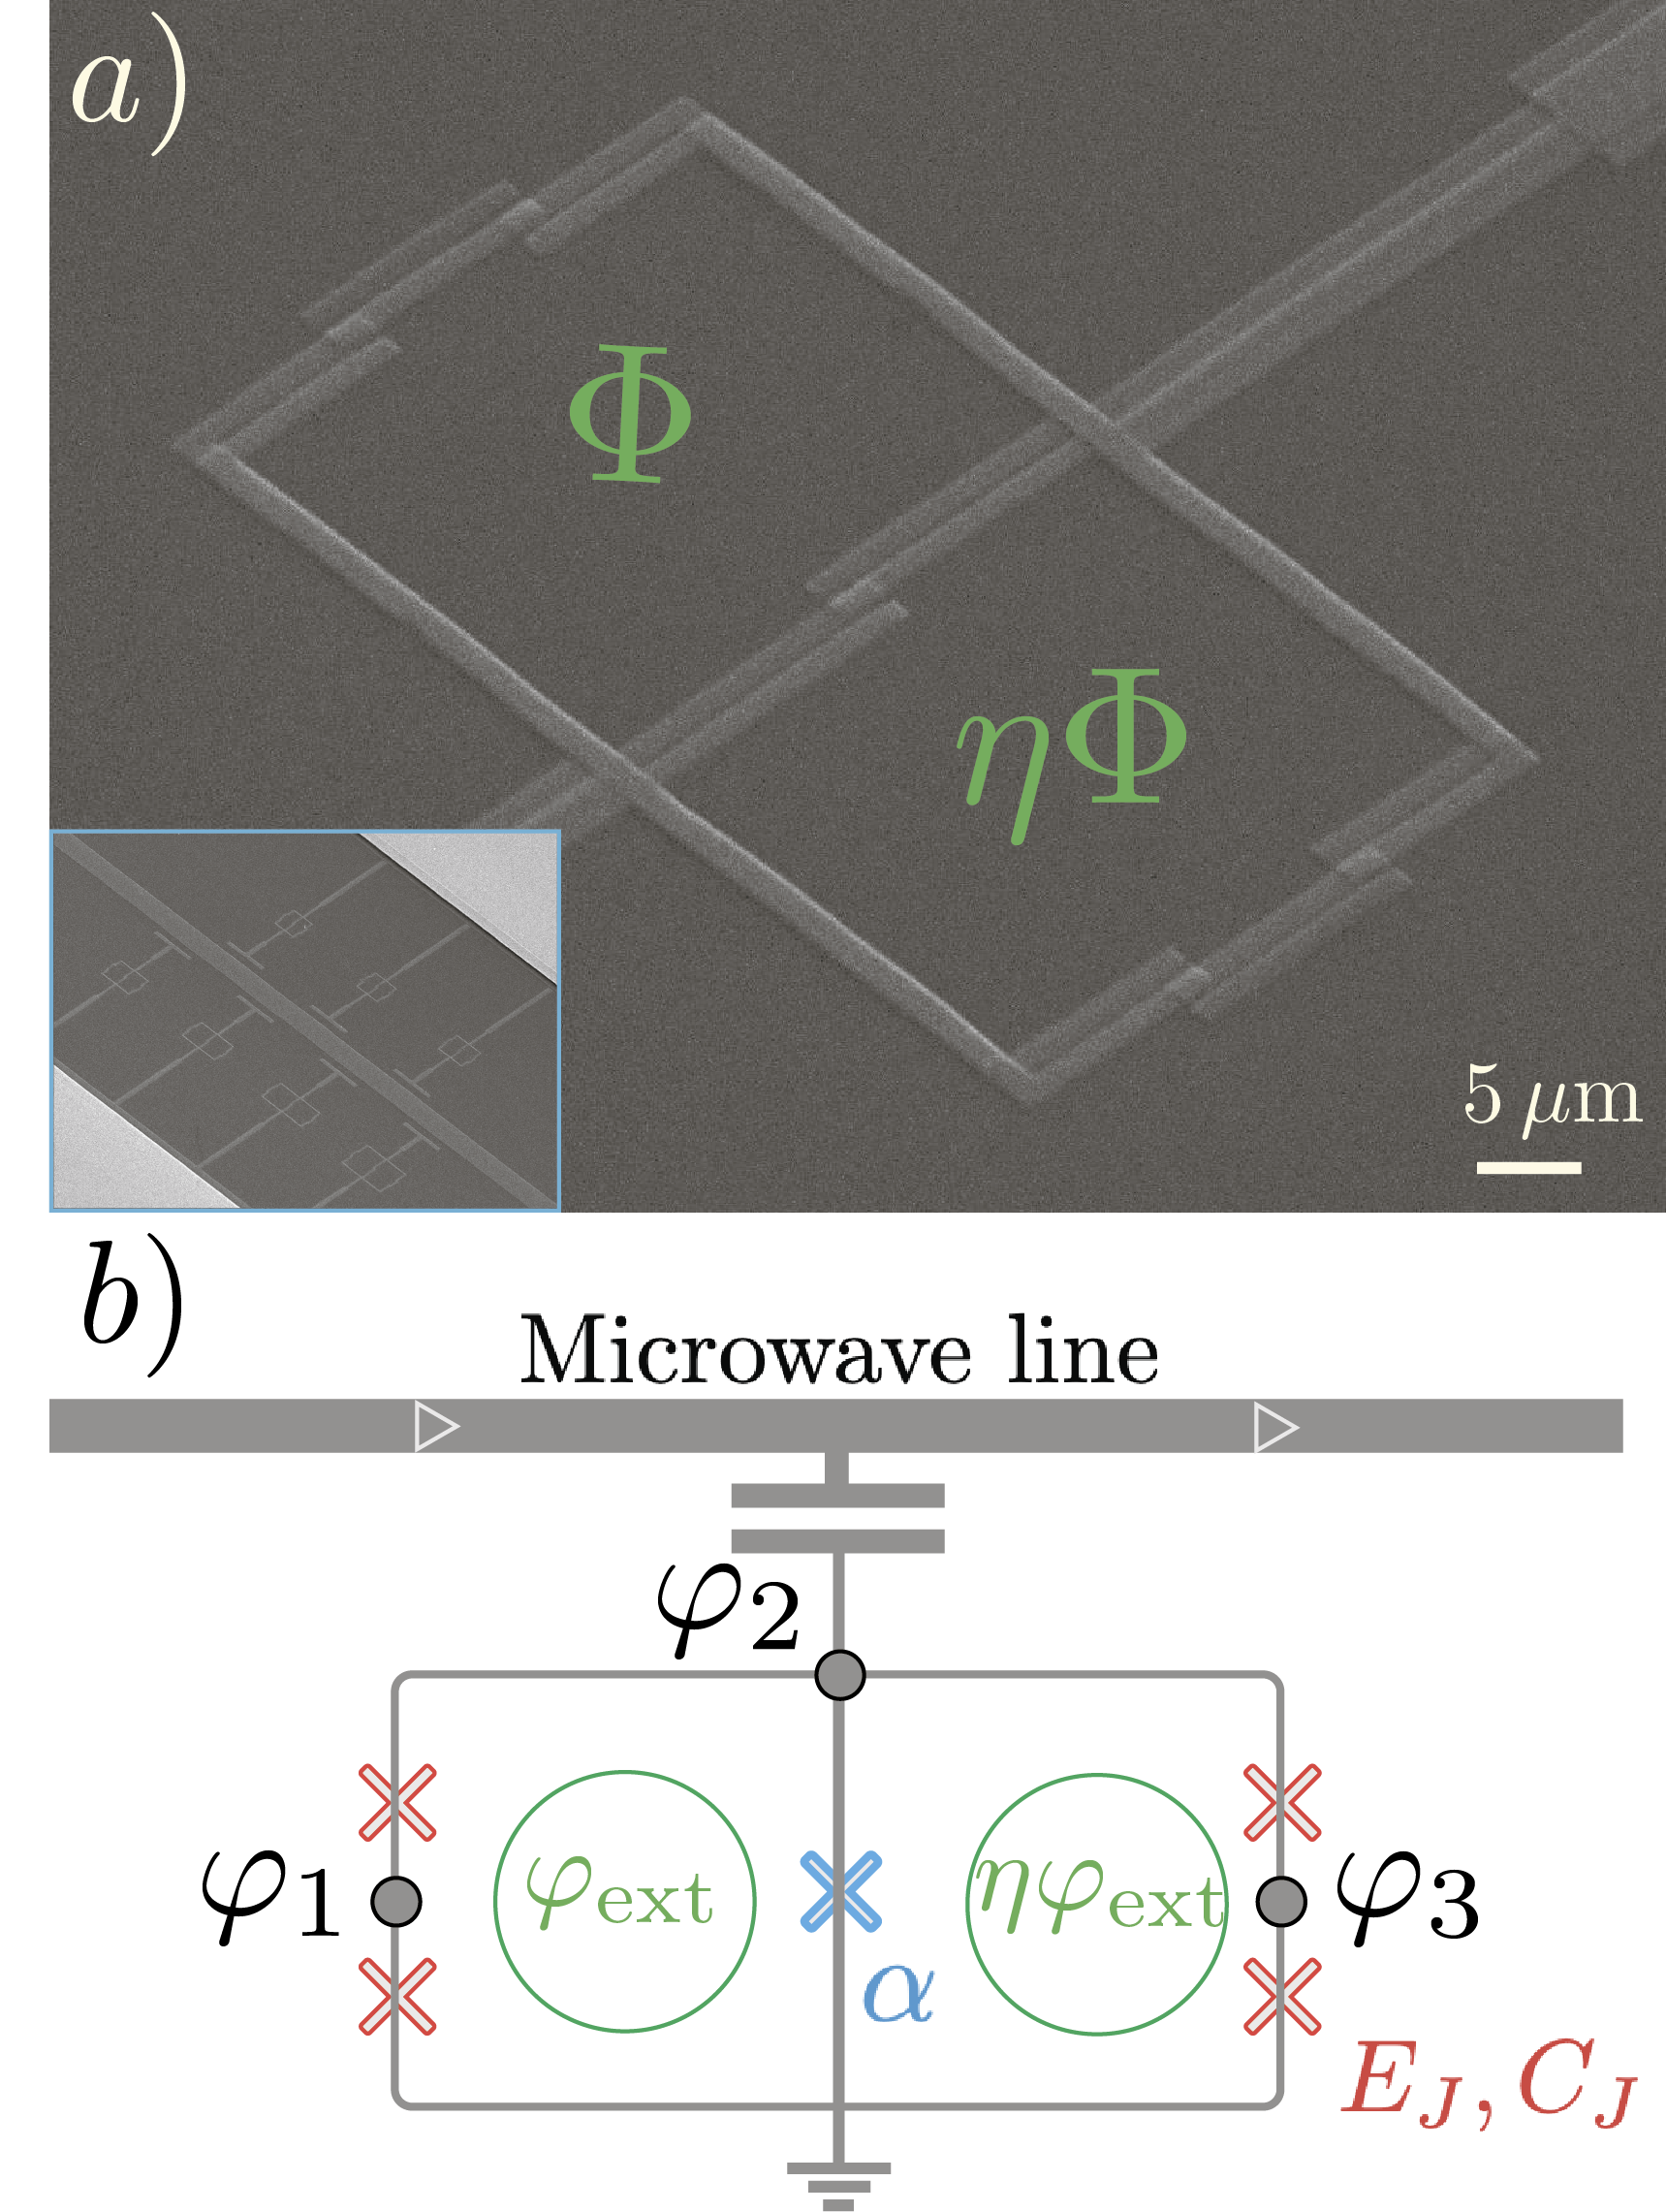
\includegraphics[height=10.5cm]{figure1_v2}
 	\caption{\small Geometry and naming conventions of a twin qubit. a) Scanning electron microscope (SEM) image of the dipole structure with labeled assymetric (through dimensionless $ \eta $) flux bias  $ \Phi $, $ \eta\Phi $ applied to it's superconducting loops. The dipoles are of a macroscopic size $ > 20\,\mu $m coupled to a $ Z_0 = \iunit{50}{$ \Omega $} $ microwave line with T-shaped capacitors (inset); b) The state of the 5 JJs are unqiuely defined by thee phases, $ \varphi_{1}, \varphi_{2}, \varphi_{3}$ and $ \varphi_0 = 0$ which we set as a refference. The central junction has boosted $ \alpha E_J $, $ \alpha C $ energies and capacitances relative to the outside JJs.}
 	%\caption{\small{Scanning electron microscope image of the dipole qubits capacitively coupled to the tranmisssion line. A common flux $ \Phi $ is applied to each loop with an external magnetic field. This magnetic field effects the phases induced across the junction$ \varphi_i$ .} Phases will arange is such a way, so that potential energy is minimised}
 	\label{fig:setup}
 \end{figure}
 
 %%Describe fabrication
 \noindent The sample is made by coating undoped silicon with gold film, and patterning out a $ Z \approxeq 50\,\Omega $ coplanar transmission line that passes through to an opening in the center of the chip. Twin qubits and T-shaped coupling capacitros are deposited in this region using shadow evaporation of aluminium with intermediate oxidation to create the 5-JJ (Fig.~\ref{fig:setup}). Measurements were performed in a 14\,mK environment to supress thermal activation and all micrwoave signals were passed through a single transmission line.
 
 %% Desribe what was measured
 The energy spectrum of Fig.~\ref{fig:experiment} is taken on the qubit whose transitions energies fell within the 1-40\,GHz frequency range of our low-noise microwave setup. An external magnetic field is applied perpendicular to the plane of the qubit, linking fluxes $ \Phi = \frac{\varphi}{2\pi}\Phi_0$ and $ \eta\Phi $ ($ \eta $ is flux bias assymetry resutling from area differences during fabrication). The
 \iket{1}$\,\rightarrow\,$\iket{2} transition (blue) is mapped by sweeping microwave signals and monitoring their tranmission on a Vector Network Analyzer (VNA). The  \iket{2}$\,\rightarrow\,$\iket{3} transition (red) is mapped using two-tone spectroscopy: a VNA is dynamically tuned to probe frequency $ \omega_{21} $, populating state \iket{2}, while an additional microwave generator passes it's own frequency, $ \omega $. Whenever it strikes the \iket{2}$ \,\rightarrow\,$\iket{3} transition ($\omega = \omega_{32} $), the depopulation of states \iket{1} and \iket{2} will result in the VNA probe, $ \omega_{21} $, passing undisturbed and reading a high transmission. For both cases we assign points onto the described transmission features to extract the energy profile of the system.
 
 %%%%%
 % image of experimental result
 %%%%%
 \begin{figure}[h!]
 	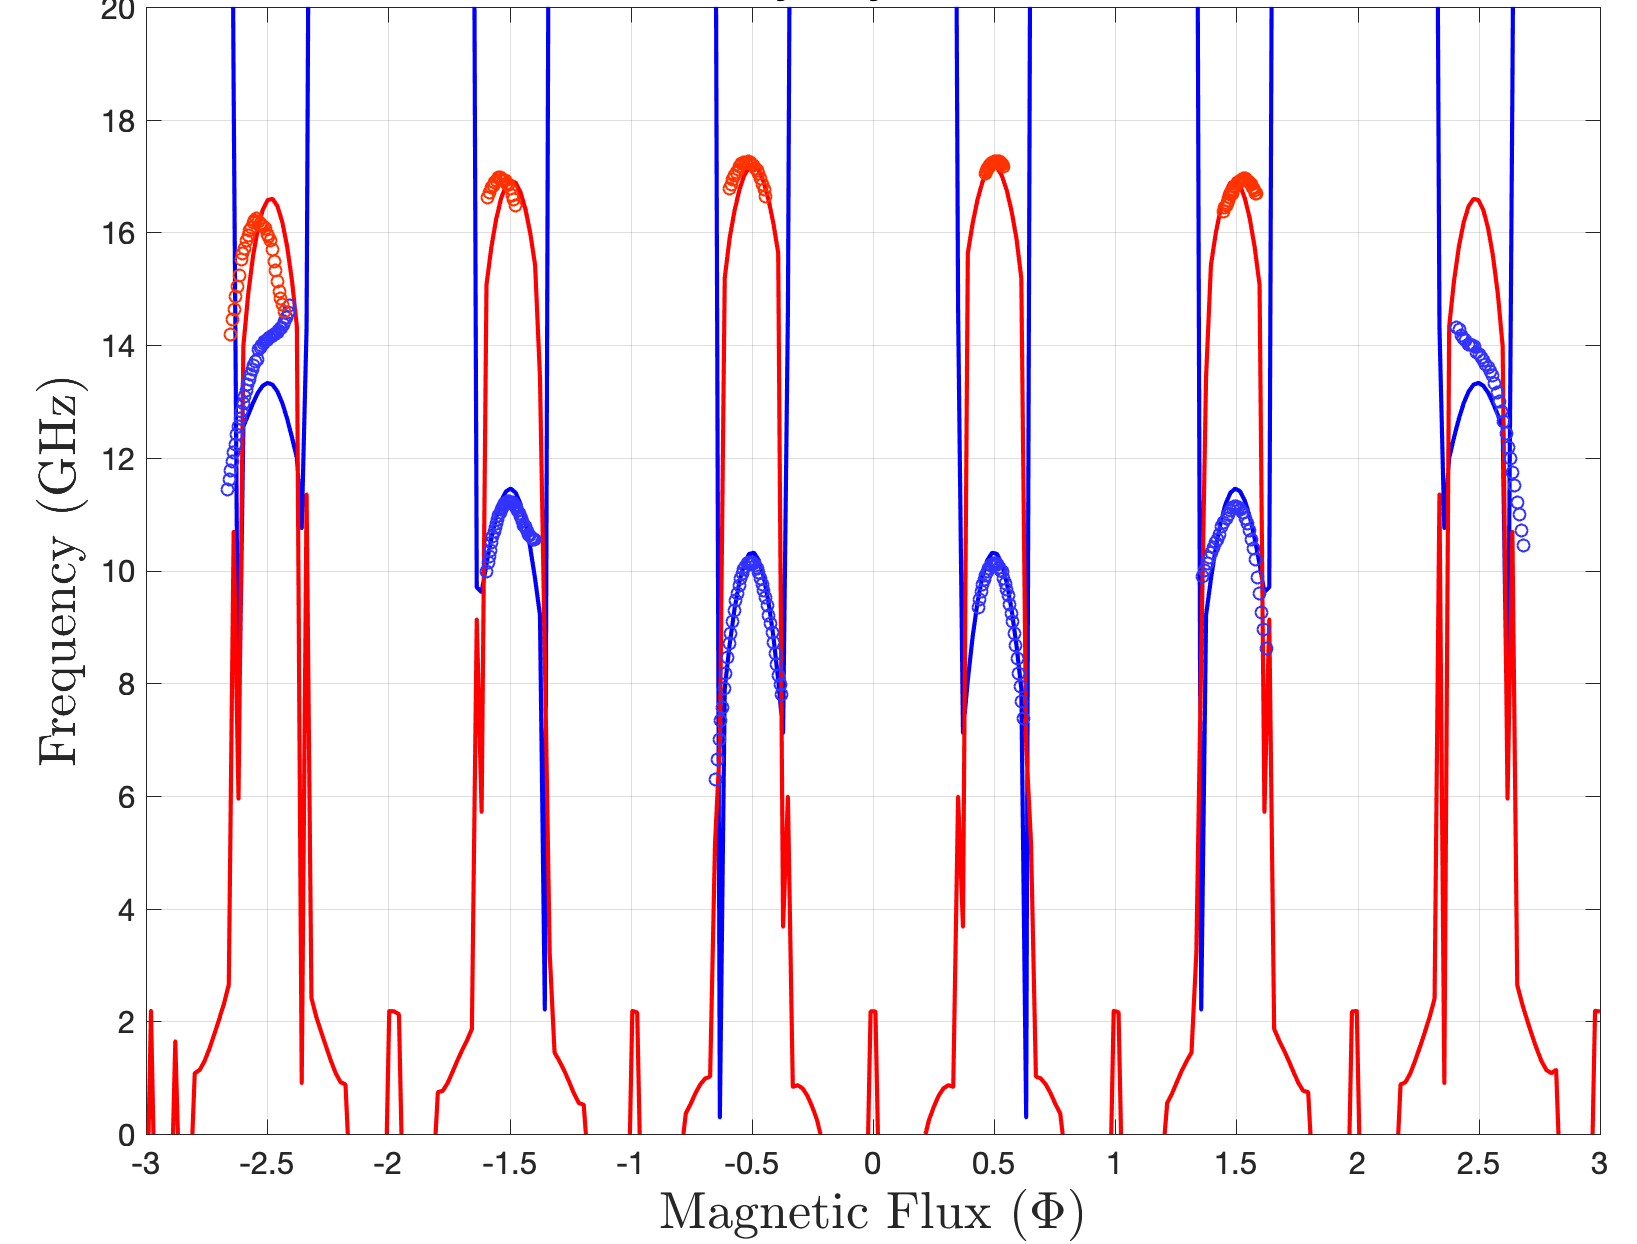
\includegraphics[height=5.5cm]{figure3_qubit2}	
 	\caption{\small Transition frequencies on the twin qubit between the lowest lying levels, $ \omega_{21} $ (blue) and $ \omega_{32}$ (red). Assymetry in the flux penetrating the left and right loops results in their gradual offset and rise away from $ \Phi = 0 $, breaking the usual $ \Phi_0 $ periodicity of flux systems. Readings for $ \omega_{32} $ are abrupt because with each step from  $ \Phi = (n + \frac{1}{2})\Phi_0, n\in\mathbb{Z} $, it gets harder to tune the VNA to $ \omega_{21} $ (as part of the two-tone spectroscopy procedure) which prevents the further mapping of $ \omega_{32} $ with the second tone.
% 		The rise of the outermost $ \omega_{21} $ transition is caused by the \red{interaction with the $ \omega_{32} $ transition}. 
 		\label{fig:experiment}}
 \end{figure}

\noindent We match the experiemental data points to simulations on the system's Hamiltonian, $ \mathcal{H} = T + V $:
\begin{itemize}
	
	\item The kinetic term arises from the electrostatic charging energy of the Cooper pairs on the capacitive elements of the JJ's:
	
	\begin{equation}\label{key}
	\begin{aligned}
	T & = \sum_{i>j}\frac{Q_iQ_j}{2C_{ij}} = \frac{(2e)^2}{2}n\hat{C}^{-1}n^{T}.
	\end{aligned}
	\end{equation}
	
	\noindent Capacitance matrix $ C=\iabs{C}\left(\begin{smallmatrix} 2 & -1 & 0\\ -1 & 2 + \alpha & -1\\ 0 & -1 & 2	\end{smallmatrix}\right)$ is derived from the topology of the system in Fig.~\ref{fig:setup}. \iabs{C} is the capacitance of the outer JJ's. $ \vec{n} = (n_1, n_2, n_3) $ is the number of Cooper pairs on each of the non-grounded islands.
	
	\item The 5 JJ's, contribute $ E_{J_i}(1-\cos(\varphi_i)) $ each to the potential term:
	\begin{equation}\label{key}
	\begin{aligned}
	U & = E_J\big[4 + \alpha - \alpha\cos(\varphi_{2}) -\cos(\varphi_{1}) -\cos(\varphi_{3}) - \\ & \qquad \cos(\varphi_{2} - \varphi_{1} - \varphi_{\text{ext}}) - \cos(\varphi_{2} - \varphi_{3} + \eta\varphi_{\text{ext}})\big].
	\end{aligned}	
	\end{equation}
	
	\noindent  We apply external fluxes $ \varphi_\text{ext} $, $ \eta\varphi_\text{ext} $ and define phases across three of the JJs, $ \vec{\varphi} = (\varphi_1, \varphi_2, \varphi_3) $. All other phases in the system are pinned from the requirement of flux quantisation, $ \sum_i^{\text{loop}} \varphi_i = 2\pi n $.
\end{itemize}

 \noindent The Hamiltonian matrix is encoded in the charge-basis, $\vec{n} $, in which the kinetic term aligns on the diagonal axis and the potential term distributes itself symmetrically on the off diagonal positions (phase operators reads $ e^{\pm i\hat{\varphi}_j} = \sum_{n_i}\ketbra{n_i\pm1}{n_i}$ \cite{phase}). Experimental data (Fig.~\ref{fig:experiment}) is fitted by evaluating the eigenenergies with \iunit{E_J = 91.0}{GHz}, \iunit{E_C = 13.50}{GHz}, \iunit{\alpha = 1.023}{}, \iunit{\eta = 1.011}{}. The assymetry value, $ \eta $, is within the same order of magnitude as the visual loop area difference of 3\% from the SEM photos.
 
 \begin{figure}[h!]
 	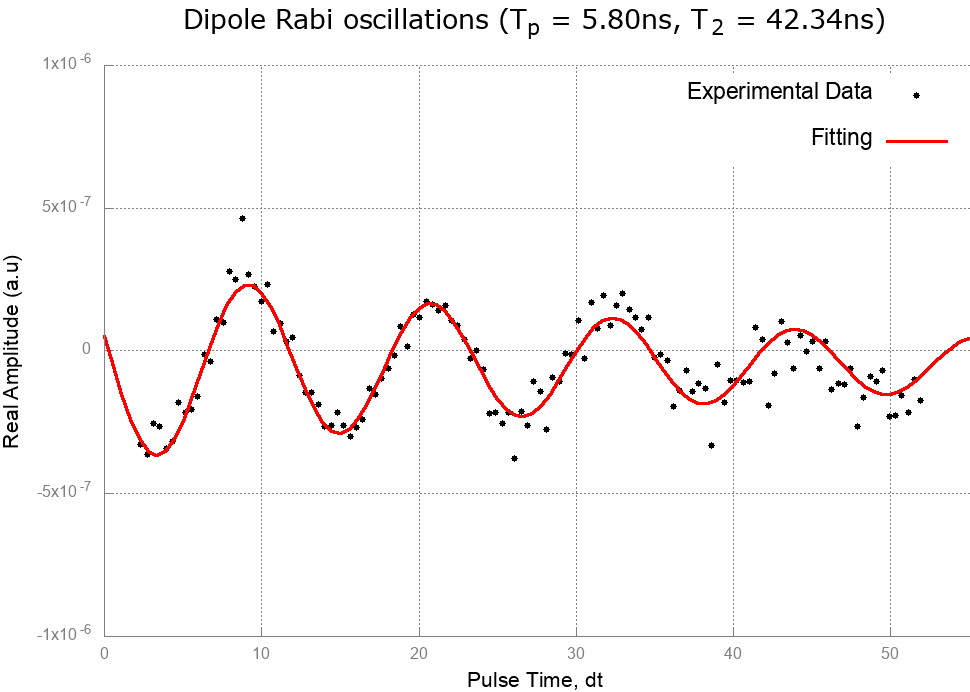
\includegraphics[height = 5cm]{figure5}
 	\caption{Rabi oscillation measurements at the degeneracy flux bias, $ \Phi_0/2 $, are made by driving the qubit with resonant microwave pulses for different time periods, $ dt $, and monitoring the signal in the output line. The a decoherence time of $ T_\varphi = \iunit{42}{ns} $ is extracted from the decay envelope, $ e^{-dt/\tau_\varphi} $, of the the oscillations. \label{fig:rabi}}
 \end{figure}

 \noindent At the degeneracy flux bias $ \sim \Phi_0(n+\frac{1}{2}), n \in \mathbb{Z} $, the energy levels posses an low curvature of $ -550\pm10\,\text{GHz}/\Phi_0^2 $ compared with $ 13\times 10^4 $ \cite{stern2014}, $ 8.4 \times 10^4 $ \cite{zhu2010}, $ 37\times 10^{4} $ \cite{gustavsson2012} $\text{GHz}/\Phi_0^2$ demonstrated in recent years on other architectures. Such broad energy level plateau makes the qubit more robust to flux noise in this operational region. A decoherence time of  $ \tau_\phi = \iunit{42}{ns} $ is extracted from Rabi oscillations, Fig.~\ref{fig:rabi}, which is high for a qubit fabricated on standard technology.
 
% \includeref{the $ T_2 = \iunit{250}{ns} $ demonstrated by other qubits}
 

